% Adjust these for the path of the theme and its graphics, relative to this file
%\usepackage{beamerthemeFalmouthGamesAcademy}
\usepackage{../../beamerthemeFalmouthGamesAcademy}
\usepackage{multimedia}
\graphicspath{ {../../} }

% Default language for code listings
\lstset{language=Python
}

% For strikethrough effect
\usepackage[normalem]{ulem}
\usepackage{wasysym}

\usepackage{algpseudocode}

\usepackage{pdfpages}

% http://www.texample.net/tikz/examples/state-machine/
\usetikzlibrary{arrows,automata}
\usetikzlibrary{tikzmark,calc}

\newcommand{\modulecode}{COMP260}\newcommand{\moduletitle}{Distributed Systems}\newcommand{\sessionnumber}{5}

\begin{document}
\title{\sessionnumber: Primitive Data Types}
\subtitle{\modulecode: \moduletitle}

\frame{\titlepage} 

\begin{frame}
	\frametitle{Learning outcomes}
	\begin{itemize}
		\item \textbf{Explain} the representation of common "plain old data" types in memory
		\item \textbf{Distinguish} pass-by-reference and pass-by-value
		\item \textbf{Distinguish} allocation of memory on the stack and on the heap
	\end{itemize}
\end{frame}

\part{Data representation}
\frame{\partpage}

\begin{frame}{Memory}
	\pause
	\begin{center}
		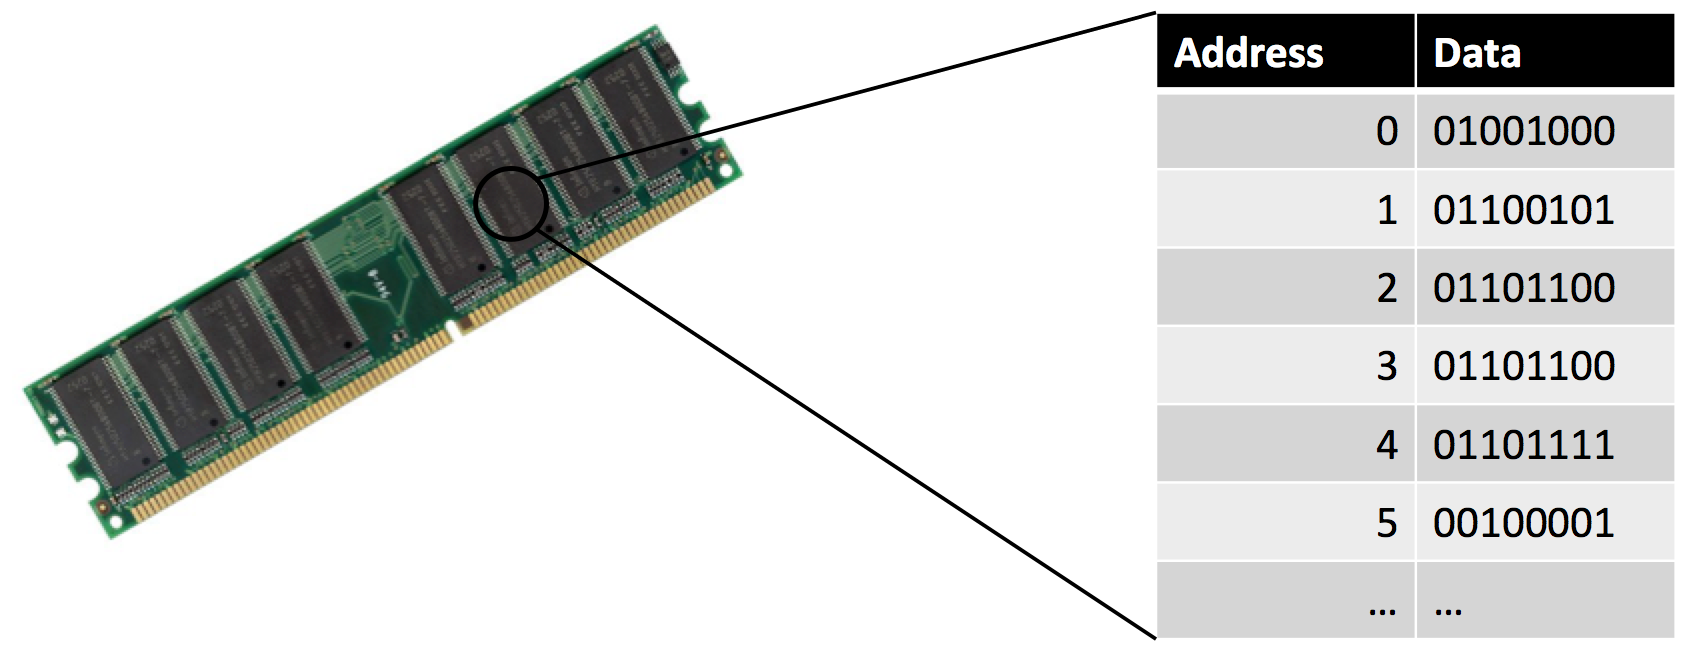
\includegraphics[width=0.8\textwidth]{memory}
	\end{center}
	\begin{itemize}
		\item Memory works like a set of \textbf{boxes}
		\pause\item Each box has a number, its \textbf{address}
		\pause\item Each box contains a \textbf{byte} (8 bits)
	\end{itemize}
\end{frame}

\begin{frame}{Data representation} 
	\begin{itemize}
		\pause\item All data is stored as \textbf{sequences of bytes}
			\begin{itemize}
				\pause\item Sequence of bits, in multiples of 8
				\pause\item Sequence of numbers between 0--255
			\end{itemize}
	\end{itemize}
\end{frame}

\begin{frame}{Number bases}
	\begin{itemize}
		\pause\item Decimal = base 10
		\pause\item Binary = base 2
		\pause\item Octal = base 8
		\pause\item Hexadecimal = base 16
			\begin{itemize}
				\pause\item Uses \texttt{A}--\texttt{F} as extra ``digits''
			\end{itemize}
		\pause\item We sometimes write the base as a \textbf{subscript}
			\begin{itemize}
				\pause\item $123_{10} = 7B_{16} = 173_{8} = 01111011_{2}$
			\end{itemize}
	\end{itemize}
\end{frame}

\begin{frame}[fragile]{Number bases in code}
	\begin{itemize}
		\pause\item In most languages (including C, C++, C\#, Python):
			\begin{itemize}
				\pause\item Decimal: \texttt{123}
				\pause\item Binary: \texttt{0b1111011}
				\pause\item Hexadecimal: \texttt{0x7B}
			\end{itemize}
		\pause\item In some languages (including C, C++, Python 2.x):
			\begin{itemize}
				\pause\item Octal: \texttt{0173}
			\end{itemize}
		\pause\item So beware of leading zeroes!
	\end{itemize}
	\begin{lstlisting}
>>> print 77
77
>>> print 077
63
	\end{lstlisting}
\end{frame}

\begin{frame}{Why is hexadecimal useful?} 
	\begin{itemize}
		\pause\item It is easy to convert between binary and hexadecimal
		\pause\item One hex digit = 4 bits
	\end{itemize}
	
	\pause $$
	\underbrace{0001}_{1}
	\underbrace{1110}_{E}
	\underbrace{0010}_{2}
	\underbrace{0100}_{4}
	\underbrace{0000}_{0}
	$$
	
	\pause So $1\,1110\,0010\,0100\,0000_{2} = 1E240_{16}$
\end{frame}

{
\setbeamercolor{background canvas}{bg=white}
\begin{frame}[plain]
	\begin{tikzpicture}[remember picture, overlay]
		\node[at=(current page.center)] {
			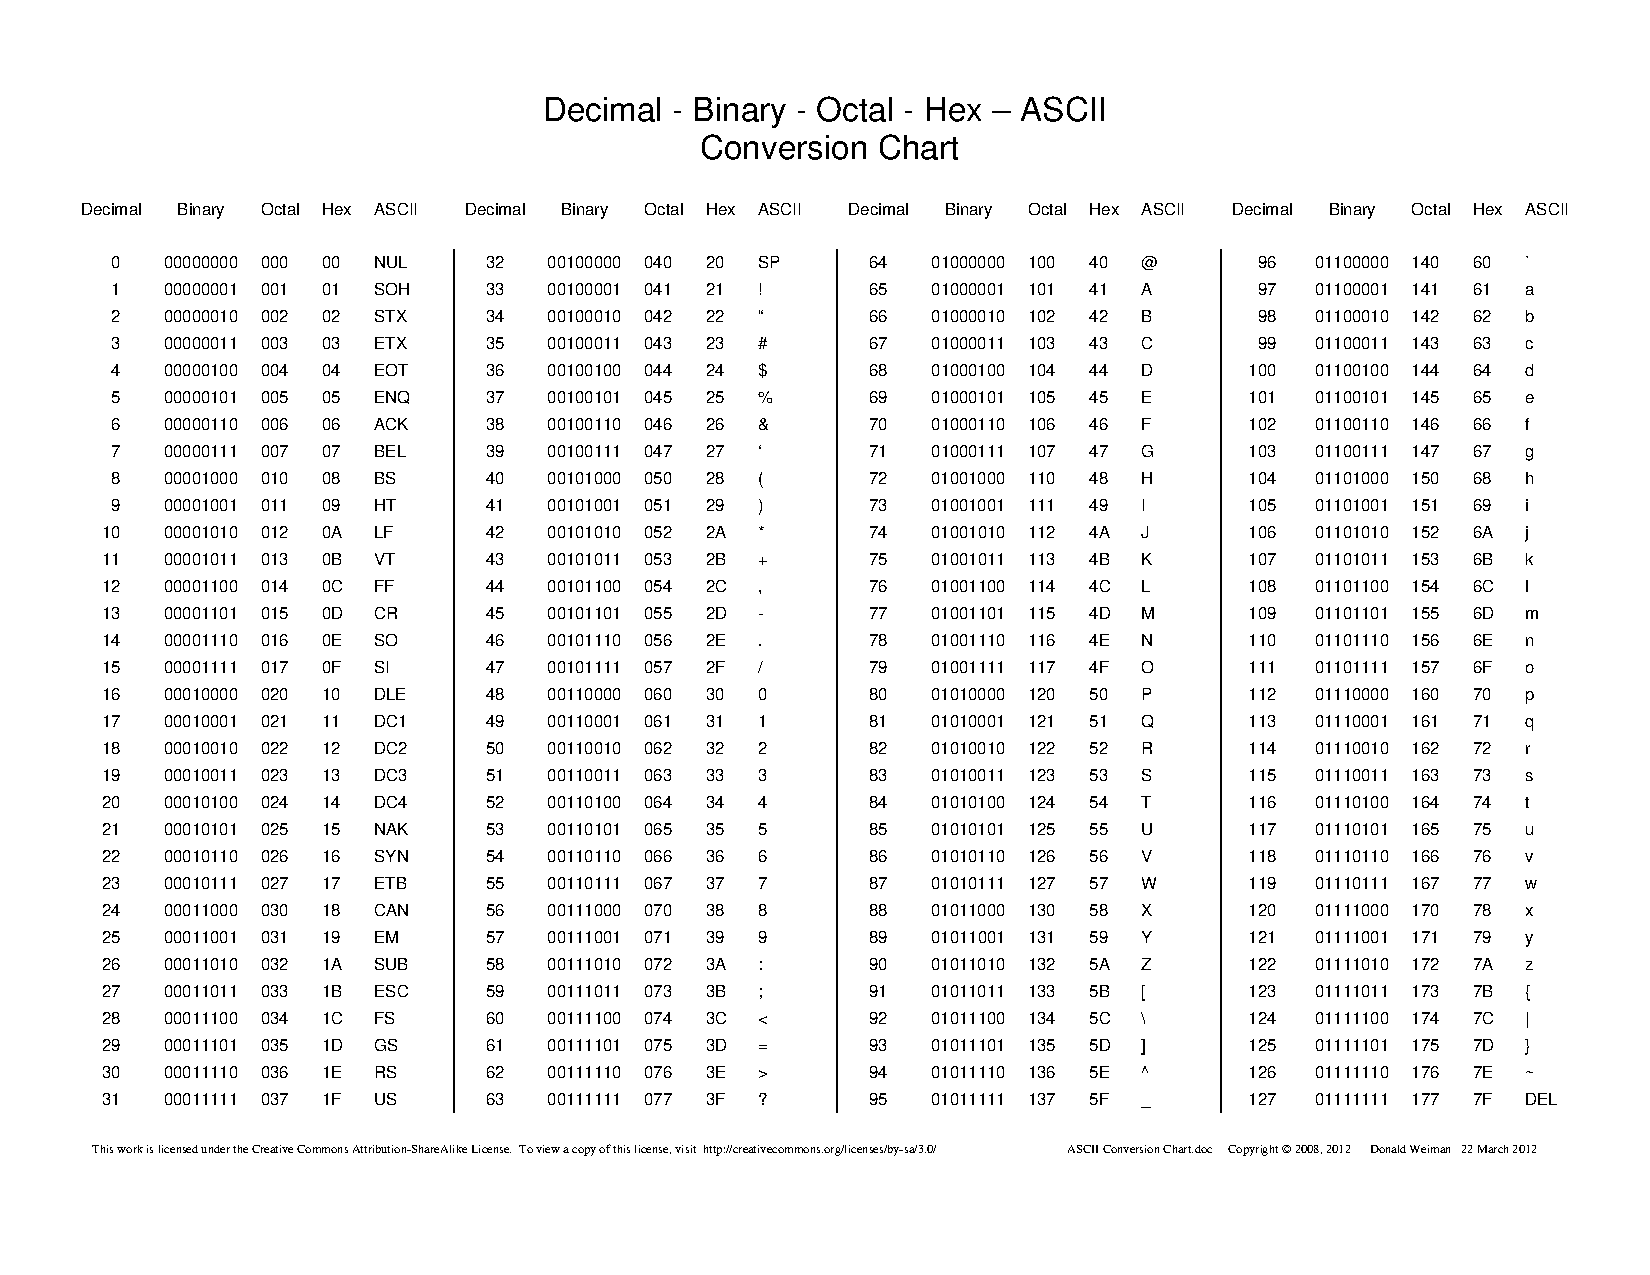
\includegraphics[width=\paperwidth]{ascii_chart}
		};
	\end{tikzpicture}
\end{frame}
}

\begin{frame}{Integers} 
	\begin{itemize}
		\pause\item Represented in \textbf{binary}
		\pause\item $n$ bits $\implies$ numbers from $0$ to $2^n-1$ inclusive
	\end{itemize}
\end{frame}

\begin{frame}{Endian-ness}
	\begin{itemize}
		\pause\item Intel x86/x64 architecture is \textbf{little endian}
		\pause\item Bytes are in ``reverse'' order (least significant first)
		\pause\item E.g.\ $123456_{10} = 1E240_{16}$, represented as
			\texttt{40 E2 01 00}
	\end{itemize}
\end{frame}


\newcommand{\socrative}{
	\begin{center}
		Socrative room code: \texttt{FALCOMPED}
	\end{center}
}

\part{Pass by reference}
\frame{\partpage}

\begin{frame}{References}
	\begin{itemize}
		\pause\item Our picture of a variable: a labelled box containing a value
		\pause\item For ``plain old data'' (e.g.\ numbers), this is accurate
		\pause\item For \textbf{objects} (i.e.\ instances of classes), variables actually hold
			\textbf{references} (a.k.a.\ \textbf{pointers})
		\pause\item It is possible (indeed common) to have \textbf{multiple references} to the same underlying object
	\end{itemize}
\end{frame}

\begin{frame}{The wrong picture}
	\begin{columns}
		\begin{column}{0.58\textwidth}
			\lstinputlisting{references_0.cs}
		\end{column}
		\pause
		\begin{column}{0.38\textwidth}
			\begin{center}
				\colorbox{white}{
					\color{black}
					\begin{tabular}{|c|c|}
						\hline
						\textbf{Variable} & \textbf{Value} \\\hline
						\texttt{x} & \uncover<3->{\begin{tabular}{|c|c|}
							\hline
							\texttt{a} & 30 \\\hline
							\texttt{b} & 40 \\\hline
						\end{tabular}} \\\hline
						\texttt{y} & \uncover<4->{\begin{tabular}{|c|c|}
							\hline
							\texttt{a} & 50 \\\hline
							\texttt{b} & 60 \\\hline
						\end{tabular}} \\\hline
						\texttt{z} & \uncover<5->{\begin{tabular}{|c|c|}
							\hline
							\texttt{a} & 50 \\\hline
							\texttt{b} & 60 \\\hline
						\end{tabular}} \\\hline
					\end{tabular}
				}
			\end{center}
		\end{column}
	\end{columns}
\end{frame}

\begin{frame}{The right picture}
	\begin{columns}
		\begin{column}{0.58\textwidth}
			\lstinputlisting{references_0.cs}
		\end{column}
		\pause
		\begin{column}{0.38\textwidth}
			\colorbox{white}{\parbox{0.9\textwidth}{
				\begin{center}
					\color{black}
					\begin{tabular}{|c|c|}
						\hline
						\textbf{Variable} & \textbf{Value} \\\hline
						\texttt{x} & \tikzmark{valuex} \\\hline
						\texttt{y} & \tikzmark{valuey} \\\hline
						\texttt{z} & \tikzmark{valuez} \\\hline
					\end{tabular}
					\par
					\vspace{3ex}
					\uncover<3->{\begin{tabular}{|c|c|}
						\hline
						\texttt{a} & \tikzmark{objectx}30 \\\hline
						\texttt{b} & 40 \\\hline
					\end{tabular}}
					\hspace{1ex}
					\uncover<4->{\begin{tabular}{|c|c|}
						\hline
						\texttt{a} & \tikzmark{objecty}50 \\\hline
						\texttt{b} & 60 \\\hline
					\end{tabular}}
				\end{center}
			}}
		\end{column}
	\end{columns}
	
\begin{tikzpicture}
		[
		  remember picture,
		  overlay,
		  -latex,
		  color=red,
		  yshift=0.5ex,
		  shorten >=1pt,
		  shorten <=1pt,
		]
		\pause\draw ({pic cs:valuex}) to [bend right] ($ ({pic cs:objectx}) + (0, 1ex) $);
		\pause\draw ({pic cs:valuey}) to [bend right] ($ ({pic cs:objecty}) + (0, 1ex) $);
		\pause\draw ({pic cs:valuez}) to [bend left] ($ ({pic cs:objecty}) + (0, 1ex) $);
	\end{tikzpicture}
\end{frame}

\begin{frame}{Values and references}
	\socrative
	\lstinputlisting{references_1.cs}
\end{frame}

\begin{frame}{Values and references}
	\socrative
	\lstinputlisting{references_2.cs}
\end{frame}

\begin{frame}{Values and references}
	\socrative
	\lstinputlisting{references_3.cs}
\end{frame}

\begin{frame}[fragile]{Pass by value}
	\socrative
	In \textbf{function parameters},
	``plain old data'' is passed by \textbf{value}
	\pause
	\begin{lstlisting}
void doubleIt(int x)
{
	x = x * 2;
}

int a = 7;
doubleIt(a);
Console.WriteLine(a);
	\end{lstlisting}
	\pause
	What does it print?
\end{frame}

\begin{frame}[fragile]{Pass by reference}
	\socrative
	However, objects (class instances) are passed by \textbf{reference}
	\pause
	\begin{lstlisting}
class Foo
{
	public int value;
	public Foo(int v) { value = v; }
}

void doubleIt(Foo x)
{
    x.value = x.value * 2;
}

Foo a = new Foo(7);
doubleIt(a);
Console.WriteLine(a.value);
	\end{lstlisting}
	\pause
	What does it print?
\end{frame}

\begin{frame}[fragile]{Lists are objects too}
	\pause
	\begin{lstlisting}
List<string> a = new List<string>{ "Hello" };
List<string> b = a;
b.Add("world");
foreach (string word in a)
{
	Console.WriteLine(word);
}
// Output:
//   Hello
//   world
\end{lstlisting}
	\pause
	... which means you should be careful when passing lists into functions,
	because the function might actually change the list!
\end{frame}

\begin{frame}[fragile]{Pass by value again}
	In C\#, struct instances are passed by \textbf{value}
	\pause
	\begin{lstlisting}
struct Foo
{
	public int value;
	public Foo(int v) { value = v; }
}

void doubleIt(Foo x)
{
    x.value = x.value * 2;
}

Foo a = new Foo(7);
doubleIt(a);
Console.WriteLine(a.value);
	\end{lstlisting}
	\pause
	This prints 7
\end{frame}

\begin{frame}{By reference or value?}
    \begin{itemize}
		\pause\item In C\#, these function arguments are passed \textbf{by value}:
			\begin{itemize}
				\pause\item Basic data types (\lstinline{int}, \lstinline{bool}, \lstinline{float} etc)
				\pause\item Instances of \lstinline{struct}s
			\end{itemize}
		\pause\item These function arguments are passed \textbf{by reference}:
			\begin{itemize}
				\pause\item Instances of \lstinline{class}es --- this includes classes built into .NET or Unity etc
				\pause\item Arguments with the \lstinline{ref} keyword attached
			\end{itemize}
		\pause\item Passing by value implies copying --- not a problem for small data values but beware of passing large structs around
    \end{itemize}
\end{frame}

\begin{frame}{References and pointers}
    \begin{itemize}
        \pause\item Some languages (e.g.\ C, C++) use \textbf{pointers}
        \pause\item Pointers are a type of reference, and have the same semantics
        \pause\item References in other languages (e.g.\ C\#, Python) are implemented using pointers
        \pause\item C++ also has something called references, which are similar but different
            (pointers can be \textbf{retargeted} whilst references cannot)
    \end{itemize}
\end{frame}

\begin{frame}{Pointers}
    \begin{itemize}
        \pause\item Recall that memory is a series of 1-byte locations, each with a numeric \textbf{address}
        \pause\item A \textbf{pointer} to something is simply the \textbf{address} at which it starts
        \pause\item When allocating a block of memory, the OS returns a pointer to the start of the block
        \pause\item When the memory is freed, any pointers into it are said to be \textbf{dangling}
        \pause\item If the memory is subsequently reused for something else, those pointers could end up
            pointing to random data
        \pause\item Again this is not really possible in Python/C\#, but a common source of bugs in C/C++
    \end{itemize}
\end{frame}


\end{document}
